% Solución propuesta (diseño)

\chapter*{Solución propuesta} \label{cap3}
\addcontentsline{toc}{chapter}{Solución propuesta}

\begin{flushright}
\begin{minipage}{7.85cm}
    {\em No podemos resolver los problemas utilizando la misma manera de pensar
    que utilizamos cuando los creamos.} \\ Albert Einstein
\end{minipage}
\end{flushright}

\vspace*{5mm}

\section*{Definición del Escenario de Simulación}

Los datos de entrada del simulador son los que llamamos {\bf Escenario}. En
ellos se define el área de simulación, tamaño de los hexágonos, las entradas de
agua, los tiempos, las personas, etc.

Toda esta información estará definida en un fichero tipo {\em clave=valor}, que
será procesado por el agente {\bf Creador} al lanzar la simulación.

\section*{Agentes en la Simulación}

En el siguiente esquema se muestran los agentes que conforman el simulador.
Algunos de ellos tienen un papel más importante que otros, destacando los
agentes {\bf Entorno} y los agentes {\bf Peatón}.

\begin{figure}[H]
 \centering
 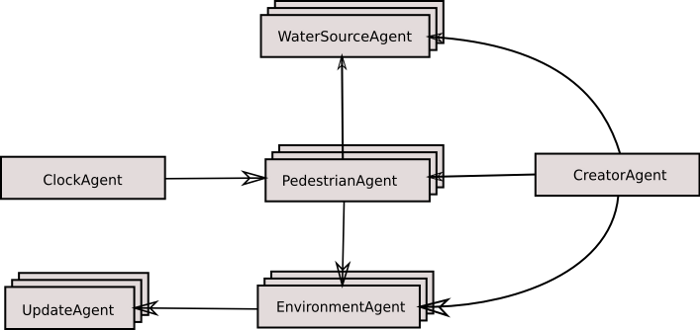
\includegraphics[width=120mm]{figuras/cap3/agents.png}
 \caption{Agentes del simulador}
\end{figure}

A continuación siguen descripciones detalladas de cada tipo de agente.

\subsection*{Agente Creador}

La función del agente Creador es la de lanzar la simulación. Esto lo convierte
en un agente un poco particular, pues no tiene un papel activo en la
simulación.

El ciclo de vida de este agente será el siguiente:

\begin{enumerate}
 \item Procesar el {\bf Escenario} de simulación.
 \item Crear los agentes {\bf Entorno}, y esperar a que hayan obtenido datos
estáticos del terreno (tales como la altura o información sobre las calles).
 \item Crear los agentes de {\bf Entrada de Agua} y los agentes {\bf Peatón}.
 \item Crear el agente {\bf Reloj} y comenzar por tanto la simulación.
 \item Quedarse a la espera por si algún agente le solicita datos del
{\bf Escenario} de simulación.
\end{enumerate}

Como se puede comprobar, una vez que el agente Creador ha terminado de lanzar
la simulación adopta un papel pasivo.

\subsection*{Agente Reloj}

La necesidad de un agente que sincronizase la simulación no se hizo patente
hasta bien avanzado el desarrollo del simulador. El motivo se explica en
profundidad en el \hyperref[cap5]{capítulo 5}.

Este agente tiene el objetivo de sincronizar al resto de agentes, y su
funcionamiento es muy sencillo. Dado un periodo de tiempo, definido en el
{\bf Escenario} de simulación, el agente Reloj ha de enviar regularmente un
mensaje al resto de agentes dando lugar a un ciclo de simulación.

Los agentes que reciben estos mensajes, y por lo tanto están sincronizados,
son: agentes {\bf Entorno}, agentes {\bf Entrada de Agua} y agentes {\bf
Peatón}.

\subsection*{Agentes Entorno}

Probablemente el agente con más responsabilidades y trabajo de todo el
simulador. Su misión es manejar la información relativa al terreno de un área
de simulación.

Para asegurar la escalabilidad del sistema ha de ser posible dividir el área a
simular entre varios agentes {\bf Entorno}, de manera que cada {\bf Entorno} se
pueda ejecutar en un núcleo diferente, o incluso en una máquina diferente. Esta
división ha de ser totalmente trasparente para los demás agentes.

Estos agentes se encargan de:

\begin{itemize}
 \item Obtener la elevación del terreno y la información relativa a calles,
puntos de interés, etc.
 \item Mover el agua de la inundación por el entorno.
 \item Recibir el agua que entre en la simulación desde un agente {\bf Entrada
de agua}.
 \item Informar a los agentes {\bf Peatón} de qué es lo que ven a su alrededor
dada su posición.
 \item Informar a los agentes {\bf Actualización} de la evolución de la
simulación.
\end{itemize}

\subsubsection*{Rejilla Hexagonal}

Para representar el terreno simulado optamos por utilizar una rejilla
hexagonal, dado que hemos de discretizar de alguna manera. El usar hexágonos
frente, por ejemplo, una cuadrícula, tiene considerables ventajas. La principal
es que la distancia del centro de un hexágono al centro de sus seis hexágonos
adyacentes es siempre la misma, mientras que en una cuadrícula esto no ocurre.

\begin{figure}[H]
 \centering
 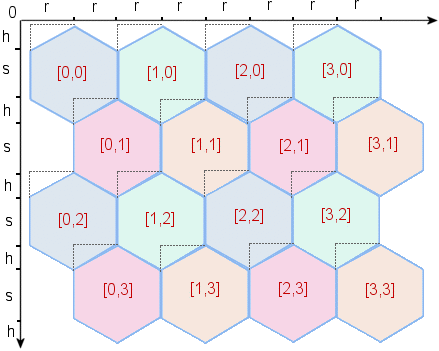
\includegraphics[width=100mm]{figuras/cap3/hexgrid.png}
 \caption{Rejilla hexagonal}
\end{figure}

Cada agente {\bf Entorno} mantiene una rejilla hexagonal con toda la
información del terreno que está simulando.

\subsection*{Agentes Entrada de Agua}

Estos agentes representan una fuente de agua del sistema. Están localizados en
un punto del área de simulación, y con cada {\em tick} del {\bf Reloj} envían
un mensaje con cierta cantidad de agua al agente {\bf Entorno} correspondiente.

La cantidad de agua de cada mensaje dependerá del ritmo de entrada de agua en
ese punto, y del ritmo de los {\em ticks} de {\bf Reloj}.

\subsection*{Agentes Peatón}

El objetivo final de toda persona que se ve envuelta un desastre es salvarse a
sí misma y a sus allegados. Ese mismo objetivo es compartido por estos agentes,
pues representan a una o a un grupo de personas.

El ciclo de vida del agente será tal que:

\begin{enumerate}
 \item Solicitar información acerca de lo que le rodea al agente {\bf
Entorno} correspondiente.
 \item Analizar dicha información y escoger una posición a la que moverse.
 \item Informar al agente {\bf Entorno} del movimiento y estado de salud.
 \item En caso de haber alcanzado algún refugio, vuelta al punto 1.
\end{enumerate}

En todo momento el agente deberá tratar, evidentemente, de no perder la vida
ahogado en la inundación.

\subsection*{Agentes Actualización}

Actúan únicamente como receptores de mensajes, su misión consiste en recibir
las actualizaciones de los agentes {\bf Entorno} y pasárselas a otros elementos
del sistema, que son los que las procesarán. Como por ejemplo, los {\bf
generadores de KML}, los {\bf visores bidimensionales} o los {\bf generadores de
estadísticas}.

En definitiva, estos agentes sirven para obtener información de la simulación
que se esté llevando a cabo.

\section*{Elevación del Terreno}

Para obtener los datos de elevación del terreno hemos de utilizar fuentes de
datos externas. En concreto para los Estados Unidos utilizaremos el servicio
web de la USGS\footnote{United States Geological Survey:
\url{http://www.usgs.gov/}}, donde proveen información de hasta $ \tfrac{1}{9} $
de segundo de arco de precisión (aproximadamente 3 metros), gracias a la base de
datos NED\footnote{National Elevation Dataset: \url{http://ned.usgs.gov/}}. Este
servicio es gratuito y de libre uso.

El simulador ha de ser totalmente independiente de la fuente de datos de
elevación, de manera que sea sencillo añadir nuevas fuentes de datos para poder
simular en territorios fuera de los Estados Unidos. De esta manera el terreno
sobre el que simular sólo estará limitado por los datos de los que dispongamos.

\section*{Geolocalización}
Para poder geolocalizar los elementos y
poder utilizarnos en nuestra simulación, necesitamos crear una equivalencia
entre casilla y coordenada.

De esta forma todo lo que simulemos podremos trasladarlo por medio de las
casillas al mundo real y toda la información del mundo real que podamos recoger
la podremos representar por medio de las casillas.

\section*{Open Street Maps}

Para la información relativa a calles, puntos de interés, etc, recurriremos a
OSM\footnote{Open Street Maps: \url{http://www.openstreetmap.org/}}. OSM es un
esfuerzo colaborativo para crear cartografía libre, es gratuito y de libre
uso\cite{Pinto09}. La calidad de los mapas en las ciudades más grandes e
importantes es muy buena, aunque en lugares menos poblados decae.

Pero al igual que con los datos de elevación, el simulador ha de ser
independiente de OSM y ha de poder utilizar otras fuentes de datos.

\section*{Generador de KML}

El generador de KML será un cliente de un agente {\bf Actualización}. Esto
significa que por cada generador de KML que esté atendiendo a la simulación
habrá un agente {\bf Actualización}. Será el agente el que mantenga la
comunicación con los agentes {\bf Entorno} que sean necesarios.

El fichero resultante deberá ser, como es natural, correcto conforme al
estándar. Para ello contamos con herramientas de
validación\footnote{Por ejemplo \url{http://www.kmlvalidator.com}} con las que
comprobar que nuestros ficheros se ajustan al estándar mantenido por el
OGC\footnote{Open Geospatial Consortium:
\url{http://www.opengeospatial.org/standards/kml}}. Es muy importante que se
ajusten al estándar para su correcta visualización en cualquier visor de KML.

\section*{Visor Bidimensional}

Se hace necesario un visor que muestre la evolución de la simulación en pseudo
tiempo real, pues estará supeditado a la frecuencia con la que reciba datos
nuevos desde los agentes {\bf Entorno}. Al igual que el {\bf generador de KML}
funcionará a través de un agente {\bf Actualización}.

El visor será bidimensional para facilitar el dibujado y reducir la carga
computacional. Deberá mostrar el estado de la simulación con cada nueva
actualización, aunque no se podrán mostrar todos los pasos dado que de aquellos
estados que ocurran entre actualización y actualización no tendrá información.

Gracias a este visor no es necesario esperar a haber completado la simulación
para poder visualizar los resultados, aunque es claramente más limitado que el
fichero KML.

\section*{Estadísticas}

También es muy importante que se puedan extraer estadísticas de las
simulaciones. Para ello usaremos, una vez más, un agente {\bf Actualización}.

Una vez generado el fichero se podrá trabajar sobre él mediante un programa
cualquiera de hojas de cálculo o similar, pudiendo generar gráficas, aplicar
fórmulas, etc.

Los datos que se almacenarán serán los relativos a las personas. Número de
muertos, de personas a salvo, etc, y el tiempo transcurrido en la simulación.
Las estadísticas que se quieran sacar se tendrán que calcular a posteriori, por
ejemplo con una hoja de cálculo, sobre los datos de estos ficheros.

%%% Local Variables:
%%% mode: latex
%%% TeX-master: "../dissim"
%%% End: